\documentclass[11pt,pdf,aspectratio=129]{beamer}
\usepackage{bibentry}
\usepackage{graphicx} % Allows including images
\usepackage{booktabs} % Allows the use of \toprule, 
\usepackage{array}
\usepackage{wrapfig}
\usepackage{graphics}
\usepackage{graphicx}
\usepackage{amsfonts}
\usepackage{amssymb}
\usepackage{amsthm}
\usepackage{textcomp}
% \usepackage{enumitem}
\usepackage{bibentry}
\usepackage{graphicx} % Allows including images
\usepackage{booktabs} % Allows the use of \toprule, 
% \usepackage[nottoc]{tocbibind}
\usepackage{threeparttable}
\usepackage{natbib}
\usepackage{mathrsfs}
\usepackage[nospace]{varioref}	
\usepackage{cleveref}

\setlength{\parskip}{\baselineskip} 
\graphicspath{{./../Figures}}
\setlength\itemsep{2em}

\usepackage{caption}
\usepackage{subcaption}


\title{Checking HANK}
\subtitle{Evidence from size-persistence tradeoff.}   
\author{\href{mailto://avlasov@nes.ru}{Vlasov Alexander}} 
\institute{NES}
\usetheme{Madrid}
% \usecolortheme{}

% \AtBeginSection{
% 	\begin{frame}
% 		\frametitle{Contents}
% 		\tableofcontents[currentsection]
% 	\end{frame}
% }

\begin{document}

\begin{frame}[fragile]
    \titlepage
\end{frame}


\section{Research question}



\begin{frame}\frametitle{Outcomes of \citet{KMV2018} model}
    \citet{KMV2018} HANK model outcomes:
    \begin{enumerate}
        \item Size-Persistence trade-off: Cumulative elasticity of aggregate consumption declines with the increase in autocorrelation of monetary shock in a nonlinear manner.
        \item Inflation-Output Tradeoff: the same Taylor rule shocks lead to the increased effects in Inflation-Output tradeoff.
    \end{enumerate}


  
\end{frame}


\begin{frame}\frametitle{Size-Persistence in RANK}
Rate path:
    \begin{equation*}
        r_t=\rho+e^{-\eta t}(r_0-\rho).\label{eq:InterestRatePath}
    \end{equation*}

NK policy    
\[C_0=\bar C\exp\left(-\frac{1}{\gamma}\int_0^\infty \left(r_s-\rho\right)\,ds\right).\]

Size:
\begin{equation*}
    R_0=\int_0^\infty \left(r_s-\rho\right)\,ds,\label{eq:KMVsize}
\end{equation*}


\[\frac{-d \log C_0}{dR_0}=\frac{1}{\gamma},\]


\end{frame}

\begin{frame}\frametitle{Picture of Size-Persistence trade-off}
    \begin{figure}\centering
        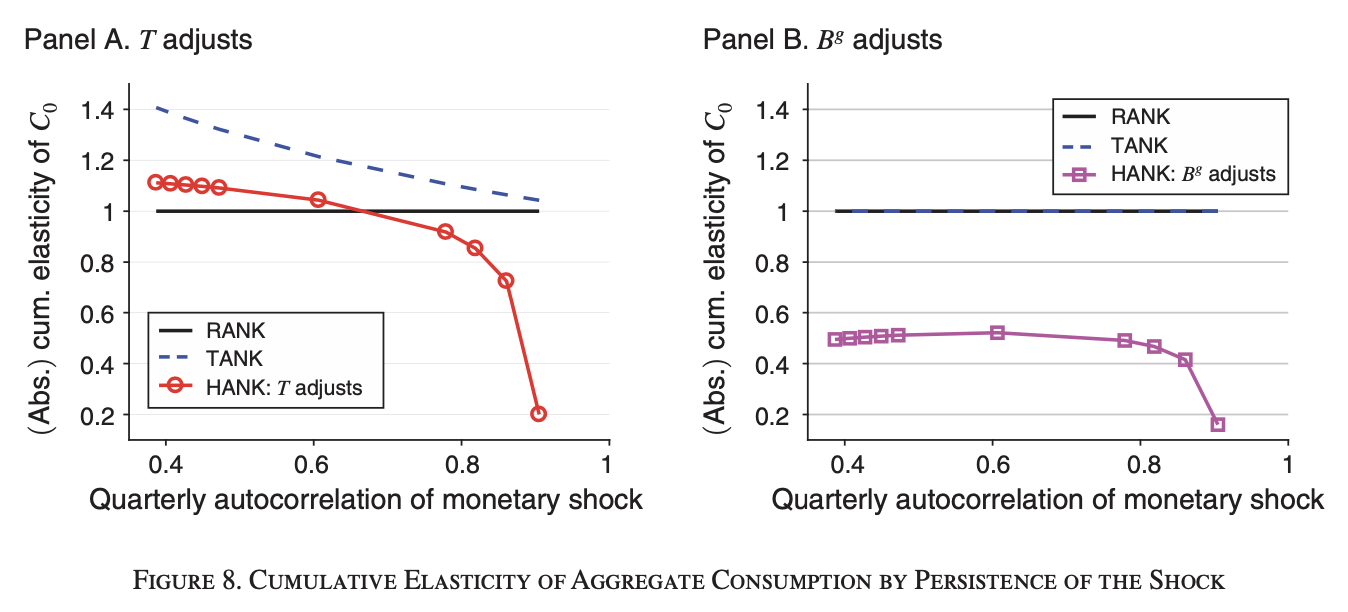
\includegraphics[scale=0.47]{Size_Persistence_KMV.png}
        \caption{The difference between the New Keynesian models from \citet{KMV2018}}
    \end{figure}
\end{frame}


\begin{frame}{Size-Persistent tradeoff by \citet{KMV2018}, formally}
    \begin{align}
        \textit{RANK:}&\quad& \frac{d}{d\nu}\frac{-d\log C_0}{dR_0}&=0     \label{eq:SizePersistenceRANK}\\
    \textit{TANK with $B^g$ adjustment:}&\quad& \frac{d}{d\nu}\frac{-d\log C_0}{dR_0}&= 0     \label{eq:SizePersistenceTANK_B}\\
    \textit{TANK with $T$ adjustment:}&\quad& \frac{d}{d\nu}\frac{-d\log C_0}{dR_0}&< 0     \label{eq:SizePersistenceTANK_T}\\
    \textit{HANK:}& \quad& 
        \frac{d^2}{d\nu ^2}\frac{-d\log C_0}{dR_0}&<0
        \label{eq:SizePersistenceHANK}
    \end{align}
    
\end{frame}


\begin{frame}\frametitle{Empirics Related to HANK}
% \begin{block}{Main work}
%     Model by \citet{KMV2018}
% \end{block}

\begin{block}{Microdata}
    \begin{itemize}
        \item \citet{HolmBlomhoff2021} find inconsistent Evidence of HANK -- the response is larger than generated by HANK.
    \end{itemize}
\end{block}
\begin{block}{MPC}
    \begin{itemize}
        \item  Estimation of MPC's\footnote{Actually MPB, but they argue that it doesn't affect the results} by \citet{Gross2020}:
        Increase of MPC is higher in 2008 than in 2011.
    \end{itemize}
\end{block}
\begin{block}{Heterogenity in Portfolios}
    \citet{Luetticke2021} find a heterogeneity in household portfolio responses to MP shocks.
\end{block}
\end{frame}


\section{Approach}

\begin{frame}\frametitle{Empirical approach:}
Based on method of \citet{HIM2023}.

I assume that the monetary policy rule is 
\[\left(r-r^*\right)_{t+h}=\tilde\phi_t\mathbb{E}\left[\pi_{t+1}\mid \mathcal{I}_t\right]+\varepsilon_t.\]
$\mathbb{E}_t\pi_{t+1}$ is the expectations of monetary authority about the inflation in quarter $t+1$.

I estimate the following State-Dependent LP-IV.
\begin{multline*}
    \left(r-r^*\right)_{t+h}=\alpha^h+\beta^h \hat\pi_t+\gamma^h \hat\pi_t\left(\mathit{Hawk}_{t}-\overline{\mathit{Hawk}}\right)\\ +\delta^h\left(\mathit{Hawk}_{t}-\overline{\mathit{Hawk}}\right)+\zeta^hZ+e_{t+h}^h,
\end{multline*}
\end{frame}

\begin{frame}{Empirical approach }

    \[\tilde \phi_{t+h}=\bar\phi+\phi_t=\hat \beta^h+\hat\gamma^h \left(\mathit{Hawk}_{t}-\overline{\mathit{Hawk}}\right).\]
    \[R_{0t}=\frac{1}{H}\sum_{h=1}^{H} \tilde \phi_{t+h}=\mathbb{E}_h \tilde \phi_{t+h}.\]
    \[\nu_t=\mathbb{E}_{h}\left[\left(\phi_{t+h}-\bar \phi\right)\left(\phi_{t+h-1}-\bar \phi\right)\right]\]

    \begin{align}
        \log \mathit{Consumption}&=\alpha_0+\alpha_1 R_0+\alpha_2\nu+\beta_1 R_0\nu \label{eq:linear}\\
        \log \mathit{Consumption}&=\alpha_0'+\alpha_1' R_0+\alpha_2'\nu+\beta_1' R_0\nu + \beta_2' R_0\nu^2\label{eq:quadratic}
    \end{align} 
\end{frame}






\section{Data}
\begin{frame}\frametitle{Data}
\begin{itemize}\setlength\itemsep{1em}
        \item Natural rate of interest by \citet{HLW2017,HLW2023}
        \item Short-term rate ($r$) is by \citet{WuXia2016} and Fed Funds Rate 
        \item Consumption is U.S. Bureau of Economic Analysis``Real personal consumption expenditures per capita ''  (FRED A794RX0Q048SBEA).
        \item FED inflation forecast is from Tealbook (average of 1 and 2 quarter ahead + average per quarter).
    \end{itemize}
\end{frame}

% \begin{frame}{Summary Statistics}
    
% \end{frame}




\section{Results}

\begin{frame}{Results I}{Policy Response to Inflation and FOMC Hawkishness}

    \begin{figure}[!htbp]\centering
        \label{fig:LP}
        \begin{subfigure}[b]{0.49\textwidth}
            \centering
            \caption{Average Response $(\beta^h)$}
            \label{fig:AverageResponce}
            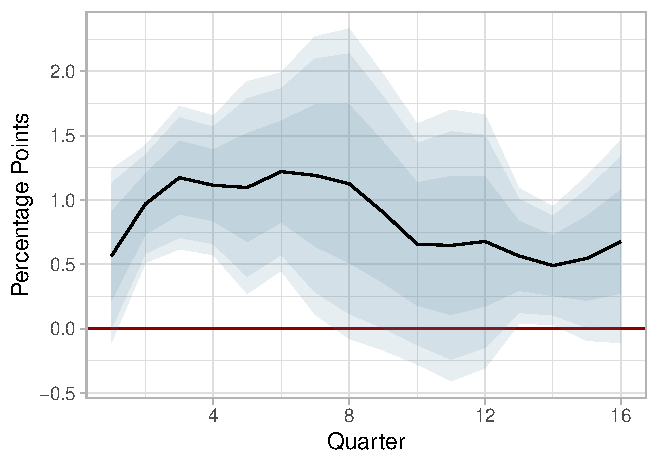
\includegraphics[width=\linewidth]{Average.pdf}
        \end{subfigure}
        \hfill
        \begin{subfigure}[b]{0.49\textwidth}
            \centering
            \caption{Differential Response $(\gamma^h)$}
            \label{fig:DifferentialResponce}
            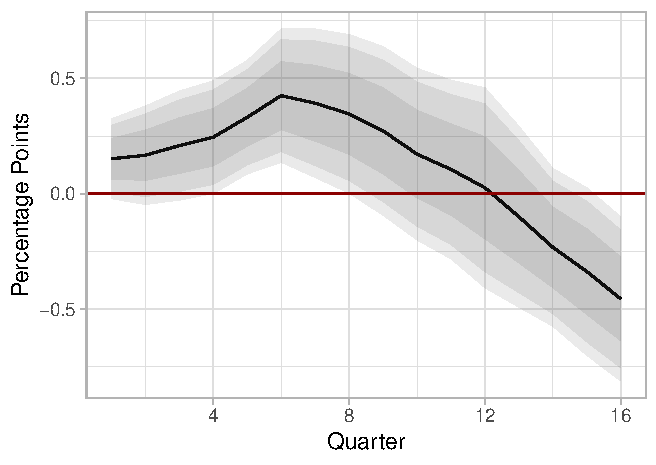
\includegraphics[width=\linewidth]{Differential.pdf}
        \end{subfigure}\vspace{-4ex}
            {\begin{flushleft}\tiny\textit{Notes}: This figure reports the responses of the $r_t-\rho_t$ to an increase in the Tealbook inflation forecast of 1 p.p. The subfigure \ref{fig:AverageResponce} reports the response for the $\mathit{HAWK}$ index equal to the sample average and \ref{fig:DifferentialResponce} is the addition to the response in case there are 2 (out of 12 in total) additional consistent hawks in the FOMC. The shaded areas correspond to 68\%, 90\% and 95\% confidence bands calculated with Newey-West HAC estimator with Andrews-selected truncation parameter.\end{flushleft}}
    \end{figure}
    
\end{frame}



\begin{frame}{Results}{Predicted IRFs}
    \begin{figure}[!htbp]\centering
        \begin{minipage}{0.7\textwidth}
          \caption{Predicted IRFs in each of the state} 
          \label{fig:predicted_IRF}
          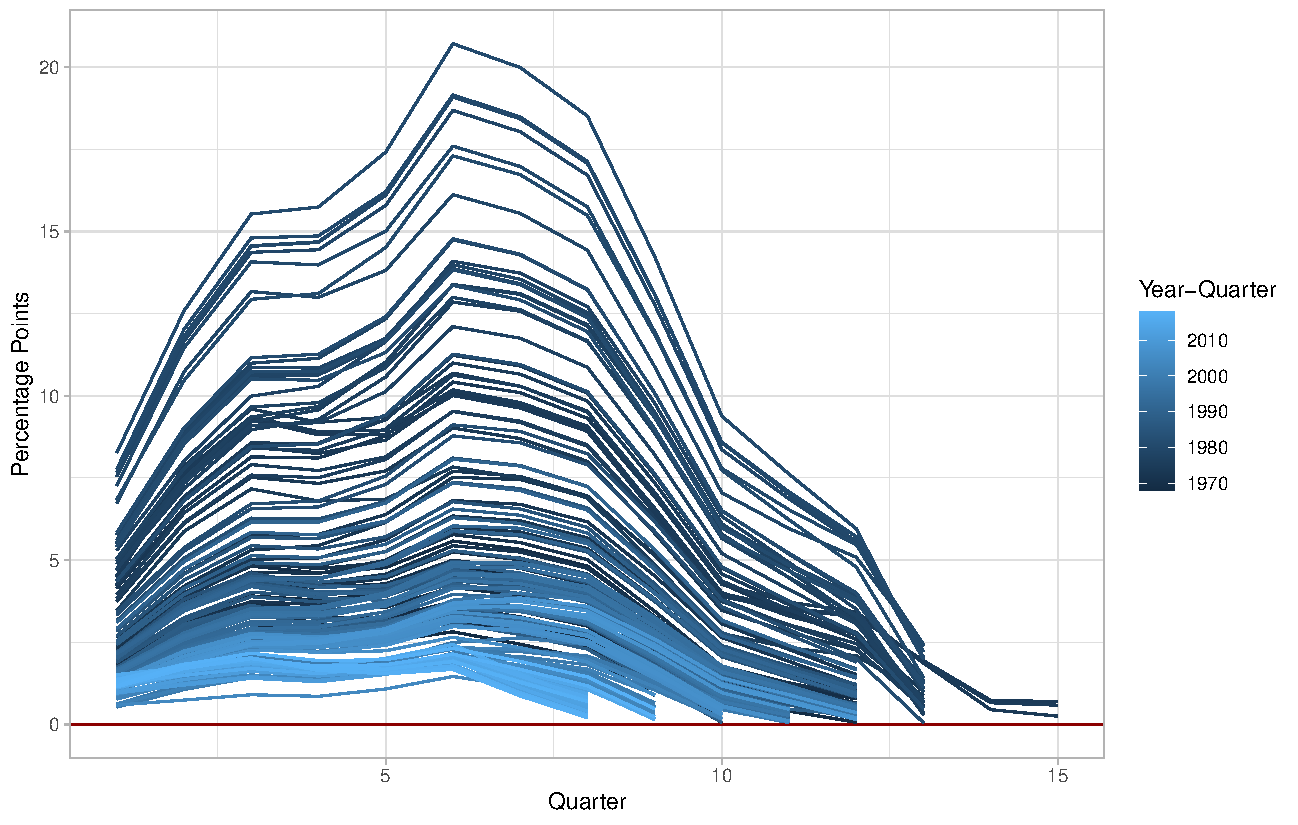
\includegraphics[width=\linewidth]{irfs_plot.pdf}
          {\begin{flushleft}\tiny \textit{Notes:} This figure shows the Impulse Response functions in each state calculated as in equation \eqref{eq:InterestRatePath}.\end{flushleft}} 
          \end{minipage}
      \end{figure}
\end{frame}


\begin{frame}{Results}{}
    \begin{figure}[!hpbt]\centering
        \begin{minipage}{0.8\textwidth}
          \caption{Estimates of Size and Persistence} 
          \label{fig:size_persistence}
          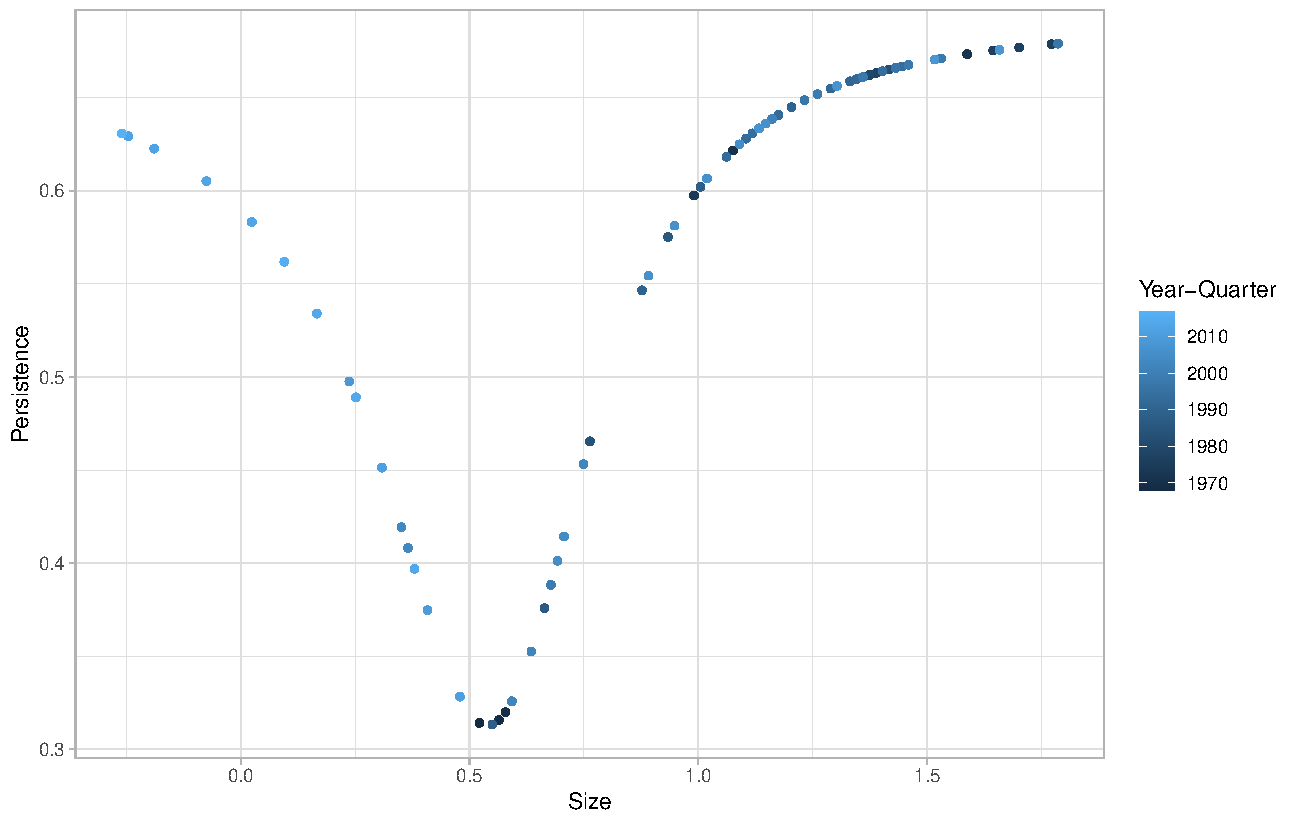
\includegraphics[width=\linewidth]{size_vs_persistence.pdf}
        %   {\begin{flushleft}\scriptsize \textit{Notes:} \end{flushleft}} 
          \end{minipage}
      
      \end{figure}
    
\end{frame}


\begin{frame}{Results}{Size and Persistence over time}
    \begin{figure}[!htbp]\centering
        \vspace{-2ex}
        \label{fig:Size_Persistence_Dynamics}
        \begin{subfigure}[b]{0.49\textwidth}
            \centering
            \caption{Size Dynamics}
            \label{fig:AverageResponce}
            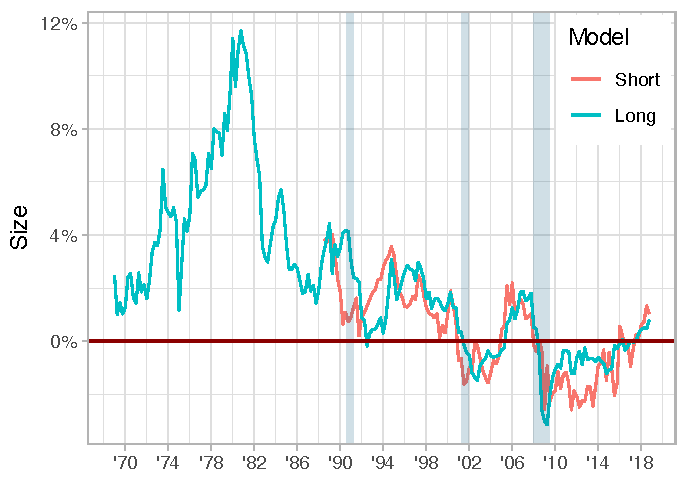
\includegraphics[width=\linewidth]{size_plot.pdf}
        \end{subfigure}
        \hfill
        \begin{subfigure}[b]{0.49\textwidth}
            \centering
            \caption{Persistence Dynamics}
            \label{fig:DifferentialResponce}
            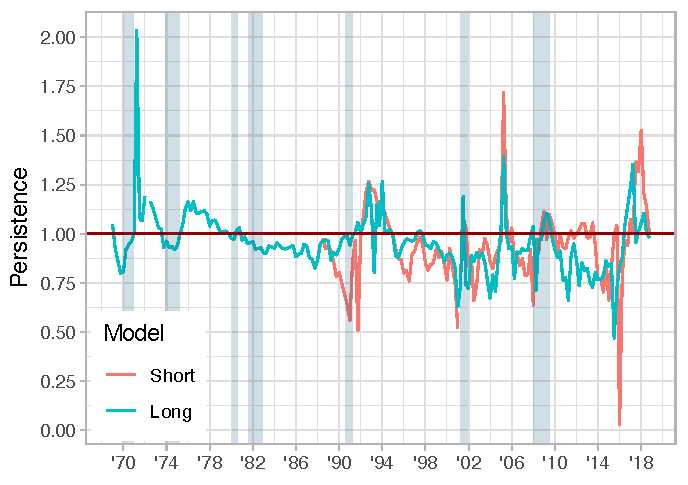
\includegraphics[width=\linewidth]{persistence_plot.pdf}
        \end{subfigure} \vspace{-5ex}
            {\begin{flushleft}\tiny\textit{Notes}: This figure presents the size and persistence, calculated as mean and the first autocorrelation of impulse-response function in each state, constructed as described in \vref{eq:InterestRatePath}, over time. \end{flushleft}}
      \end{figure}
      
\end{frame}

\begin{frame}{Results:}{Size-Persistence Tradeoff}\tiny\vspace{-2ex}
\begin{table}[!htb] \centering 
    \begin{threeparttable}
    \begin{tabular}{@{\extracolsep{10pt}}lcc} 
      \\[-1.8ex]\hline 
      \hline \\[-1.8ex] 
       & \multicolumn{2}{c}{\textit{Dependent variable:}} \\ 
      \cline{2-3} 
      \\[-1.8ex] & \multicolumn{2}{c}{$\log(\mathit{consumption})$} \\  \\[-1.8ex]   &\multicolumn{2}{c}{$H=8$}\\
      \\[-1.8ex] & (1) & (2)\\ 
      \hline \\[-1.8ex] 
       Size $(R_0)$  & $-$0.687 & $-$0.451 \\ 
        & ($-$1.149, $-$0.133) & ($-$1.495, 1.078)    \\ 
        &[0.011]\{0.997\} & [0.857]\{0.578\}\\ 
        & & \\ 
       Persistence $(\nu)$ & $-$0.100 & 1.223 \\ 
        & ($-$0.693,  0.691)   & ($-$3.598, 4.968)    \\ 
        &[0.746]\{0.673\} & [0.517]\{0.246\}\\ 
        & & \\ 
        $\nu^2$ &  & $-$1.042 \\ 
        &  &  ($-$4.271, 4.336) \\ 
        & &[0.517]\{0.766\} \\ 
        & & \\ 
       $R_0\times \nu$ & 0.765 & $-$1.628 \\ 
        & ($-$0.177,  1.526)    &   ($-$3.159,  2.748)     \\ 
        &[0.0754]\{0.0247\} & [0.522]\{0.759\}\\ 
        & & \\ 
        $R_0\times \nu^2$ &  & 2.435 \\ 
        &  &  ($-$1.852, 3.838) \\ 
        & & [0.340]\{0.145\}\\ 
        & & \\ 
       Constant & 10.6 &10.5 \\ 
        & (10.1, 11.0) & (9.8, 11.0)    \\ 
        & [0.0]\{0.0\}& [0.0]\{0.0\}\\ 
        & & \\[-1.8ex] 
      \hline \\[-1.8ex] 
      Observations & 198 & 198 \\ 
      \hline 
      \hline \\[-1.8ex] 
      \end{tabular} 
    \begin{tablenotes}[flushleft]
    \item[] \tiny \textit{Note:} The inference is derived from Block bootstrap with 10,000 replications and block lengths geometrically distributed with mean $16$. 95\% percentile intervals are in parenthesis. Bootstrap p-values for the two-sided hypothesis ($\mathbb{H}_0:\theta=0$ vs $\mathbb{H}_a:\theta\ne 0$) are in square brackets, p-values for the one-sided hypothesis ($\mathbb{H}_0:\theta=0$ vs $\mathbb{H}_a:\theta>0$) are in curly brackets. 
  \end{tablenotes}
\end{threeparttable}
  \end{table} 

\end{frame}


\section{Conclusion}
\begin{frame}\frametitle{Conclusions}
    \begin{block}{So, should we believe in HANK?}
        The evidence above suggests that, we should. 
        At least we have found that consumption behaviour in size-persistent tradeoff corresponds to the TANK model.
    \end{block}
\end{frame}





%Thanks
\begin{frame}

\begin{center}
    \Large Place for your suggestions and comments!
\end{center} 
\begin{center}
    \footnotesize
If you have any other suggestions/comments  please write \href{mailto://avlasov@nes.ru}{avlasov@nes.ru}
\end{center}


\end{frame}



\begin{frame}[t, allowframebreaks]
    \frametitle{References}
   \bibliography{../misc/references.bib}
    \bibliographystyle{../misc/econ.bst}
    \end{frame}
\end{document}